\hypertarget{index_introduction}{}\section{Introduction}\label{index_introduction}
software to collect weather data contributed by citizens; to make these data available for weather services and homeland security; to provide feedback to the data contributors so that they have the tools to check and improve their data quality

\href{http://rmap.cc}{\tt http\+://rmap.\+cc}\hypertarget{index_howto}{}\section{Howto}\label{index_howto}
\hypertarget{index_stima_ethernet}{}\subsection{S\+T\+I\+M\+A over Ethernet\+:}\label{index_stima_ethernet}
 
\begin{DoxyImageNoCaption}
  \mbox{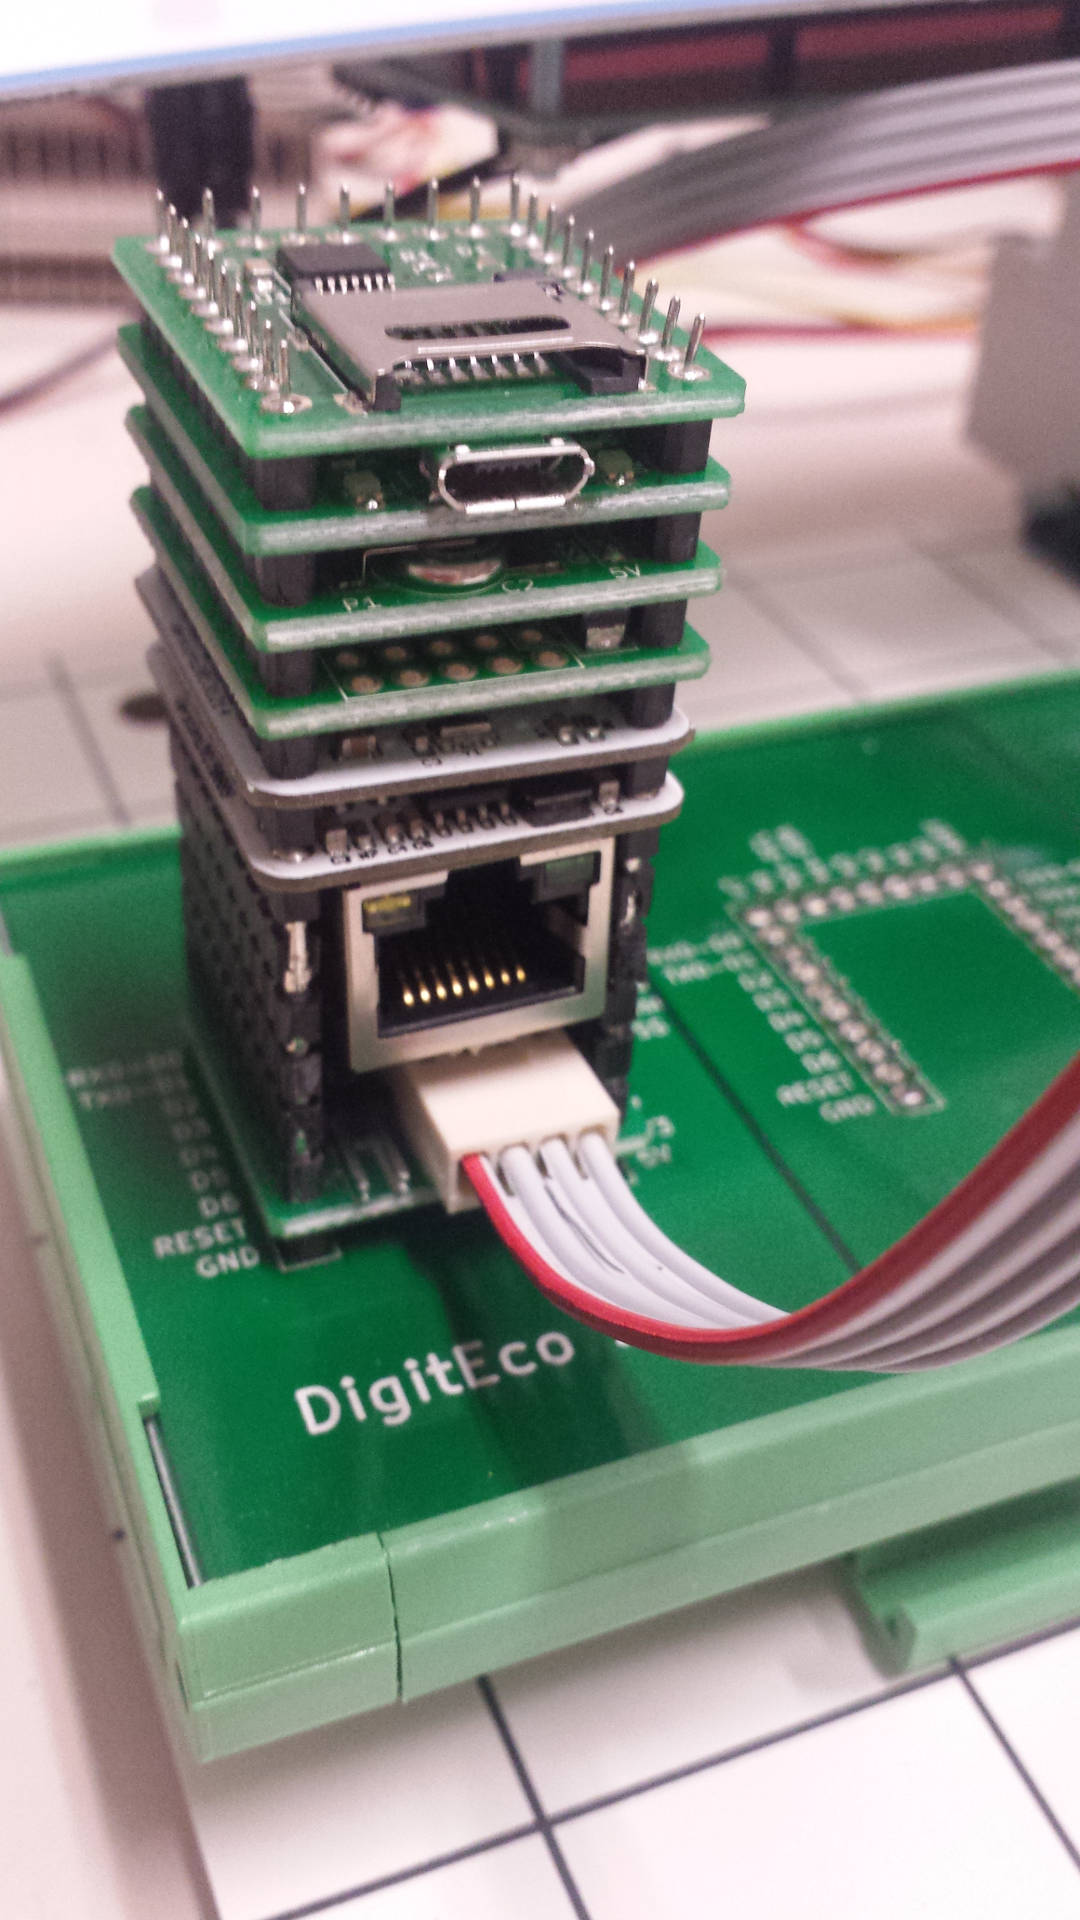
\includegraphics[width=\textwidth,height=\textheight/2,keepaspectratio=true]{ethernet.jpg}}
\end{DoxyImageNoCaption}
\hypertarget{index_stima_ethernet_hardware}{}\subsubsection{Hardware}\label{index_stima_ethernet_hardware}
1) Stima I2\+C-\/\+Base @ 5V

2) Microduino Ethernet W\+IZ

3) Microduino R\+J45

4) Stima core+1284 @ 5V

5) Stima I2\+C-\/\+R\+TC @ 5V

6) Stima F\+T232\+RL

7) Stima S\+D-\/\+Card\hypertarget{index_stima_ethernet_software}{}\subsubsection{Software}\label{index_stima_ethernet_software}
1) open sketch \hyperlink{rmap_8ino}{arduino/sketchbook/rmap/rmap/rmap.\+ino}

2) in \hyperlink{rmap-config_8h}{arduino/sketchbook/rmap/rmap/rmap-\/config.\+h} set S\+T\+I\+M\+A\+\_\+\+M\+O\+D\+U\+L\+E\+\_\+\+T\+Y\+P\+E\+\_\+\+R\+E\+P\+O\+R\+T\+\_\+\+E\+TH or S\+T\+I\+M\+A\+\_\+\+M\+O\+D\+U\+L\+E\+\_\+\+T\+Y\+P\+E\+\_\+\+S\+A\+M\+P\+L\+E\+\_\+\+E\+TH in M\+O\+D\+U\+L\+E\+\_\+\+V\+E\+R\+S\+I\+ON define

3) open \hyperlink{sensors__config_8h}{arduino/sketchbook/libraries/\+Rmap\+Config/sensors\+\_\+config.\+h} and set true or false sensors\textquotesingle{}s define and json\textquotesingle{}s define in order to enable or disable relative sensor\textquotesingle{}s driver and library

4) compile and upload firmware

5) short-\/circuit the two configure pins with a jumper and configure it!\hypertarget{index_stima_gsm}{}\subsection{S\+T\+I\+M\+A over G\+S\+M/\+G\+P\+R\+S\+:}\label{index_stima_gsm}
 
\begin{DoxyImageNoCaption}
  \mbox{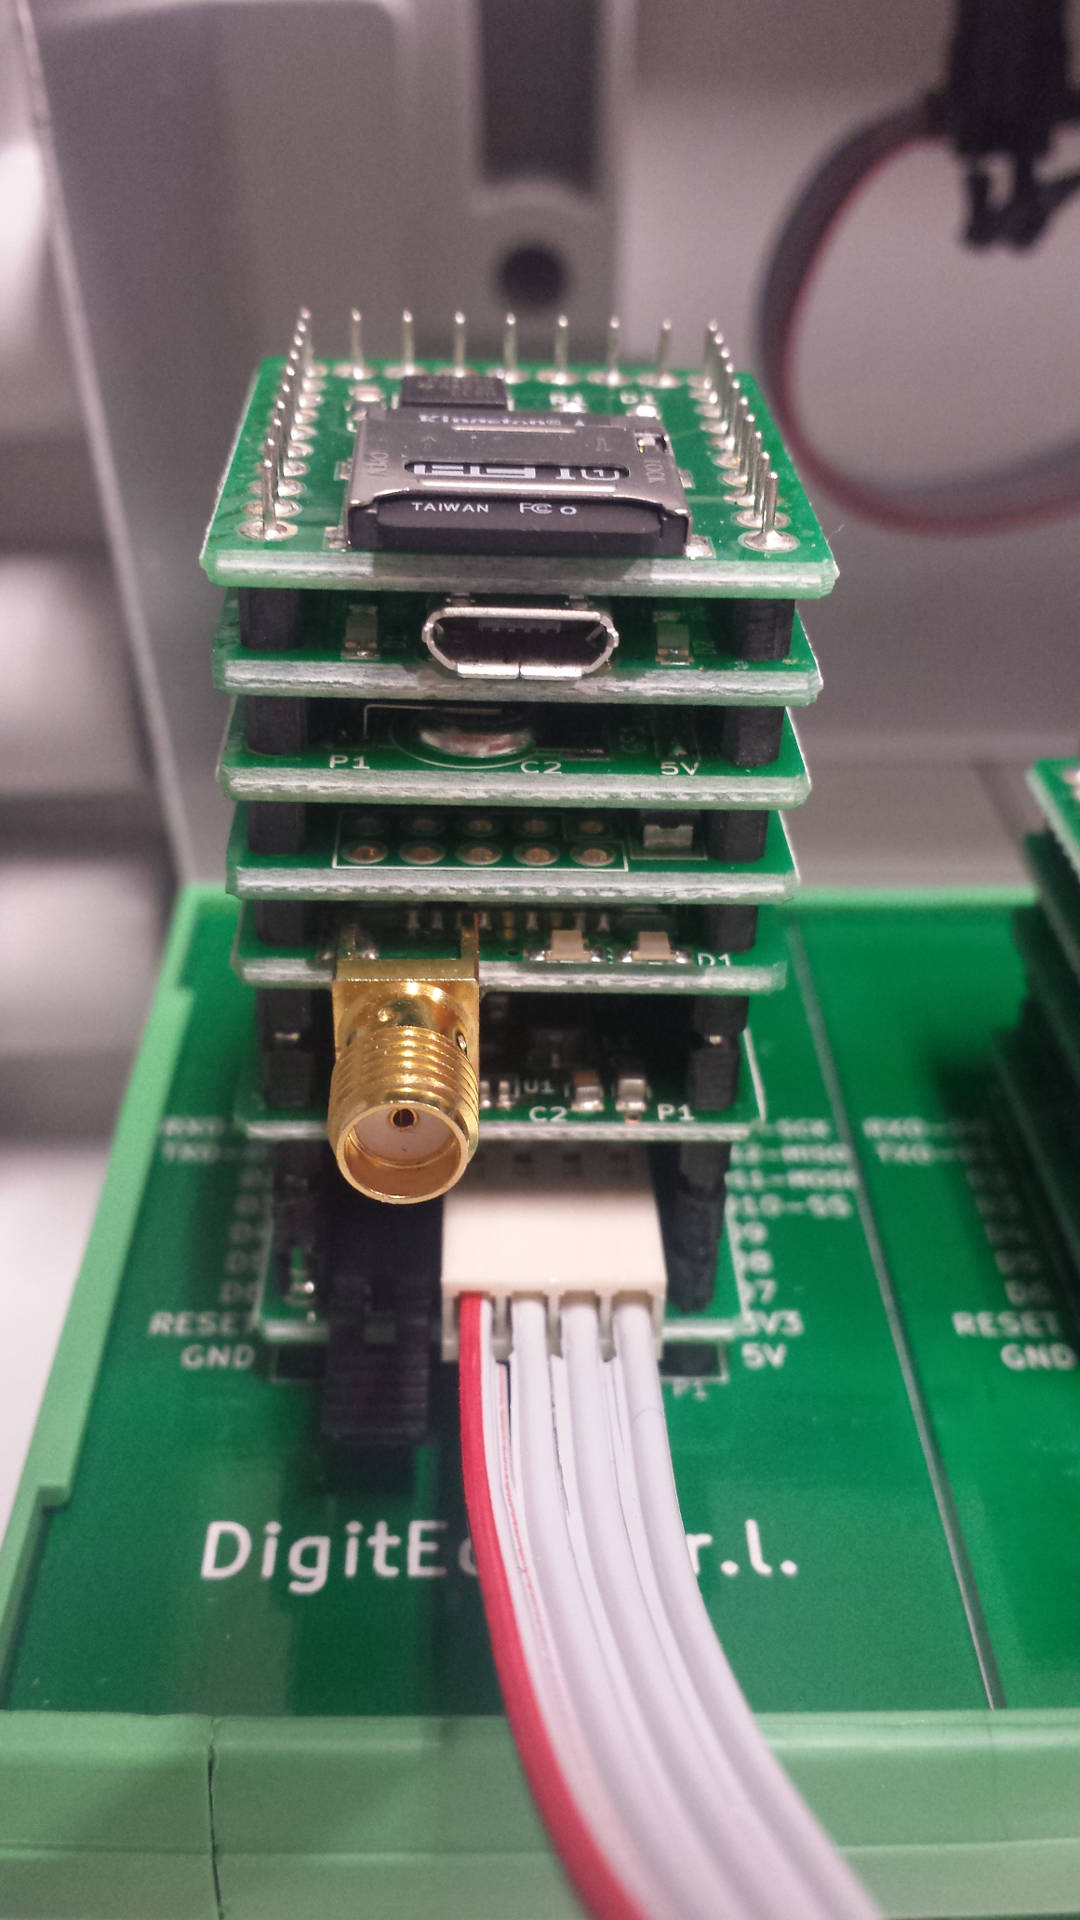
\includegraphics[width=\textwidth,height=\textheight/2,keepaspectratio=true]{gsm.jpg}}
\end{DoxyImageNoCaption}
\hypertarget{index_stima_gsm_hardware}{}\subsubsection{Hardware}\label{index_stima_gsm_hardware}
1) Stima I2\+C-\/\+Base @ 5V

2) Stima S\+I\+M800C Power

3) Stima S\+I\+M800C Module

4) Stima core+1284 @ 5V

5) Stima I2\+C-\/\+R\+TC @ 5V

6) Stima F\+T232\+RL

7) Stima S\+D-\/\+Card\hypertarget{index_stima_gsm_software}{}\subsubsection{Software}\label{index_stima_gsm_software}
1) open sketch \hyperlink{rmap_8ino}{arduino/sketchbook/rmap/rmap/rmap.\+ino}

2) in \hyperlink{rmap-config_8h}{arduino/sketchbook/rmap/rmap/rmap-\/config.\+h} set S\+T\+I\+M\+A\+\_\+\+M\+O\+D\+U\+L\+E\+\_\+\+T\+Y\+P\+E\+\_\+\+R\+E\+P\+O\+R\+T\+\_\+\+G\+SM or S\+T\+I\+M\+A\+\_\+\+M\+O\+D\+U\+L\+E\+\_\+\+T\+Y\+P\+E\+\_\+\+S\+A\+M\+P\+L\+E\+\_\+\+G\+SM in M\+O\+D\+U\+L\+E\+\_\+\+V\+E\+R\+S\+I\+ON define

3) open \hyperlink{sensors__config_8h}{arduino/sketchbook/libraries/\+Rmap\+Config/sensors\+\_\+config.\+h} and set true or false sensors\textquotesingle{}s define and json\textquotesingle{}s define in order to enable or disable relative sensor\textquotesingle{}s driver and library

4) compile and upload firmware

5) short-\/circuit the two configure pins with a jumper and configure it!\hypertarget{index_stima_passive}{}\subsection{S\+T\+I\+M\+A Passive\+:}\label{index_stima_passive}
 
\begin{DoxyImageNoCaption}
  \mbox{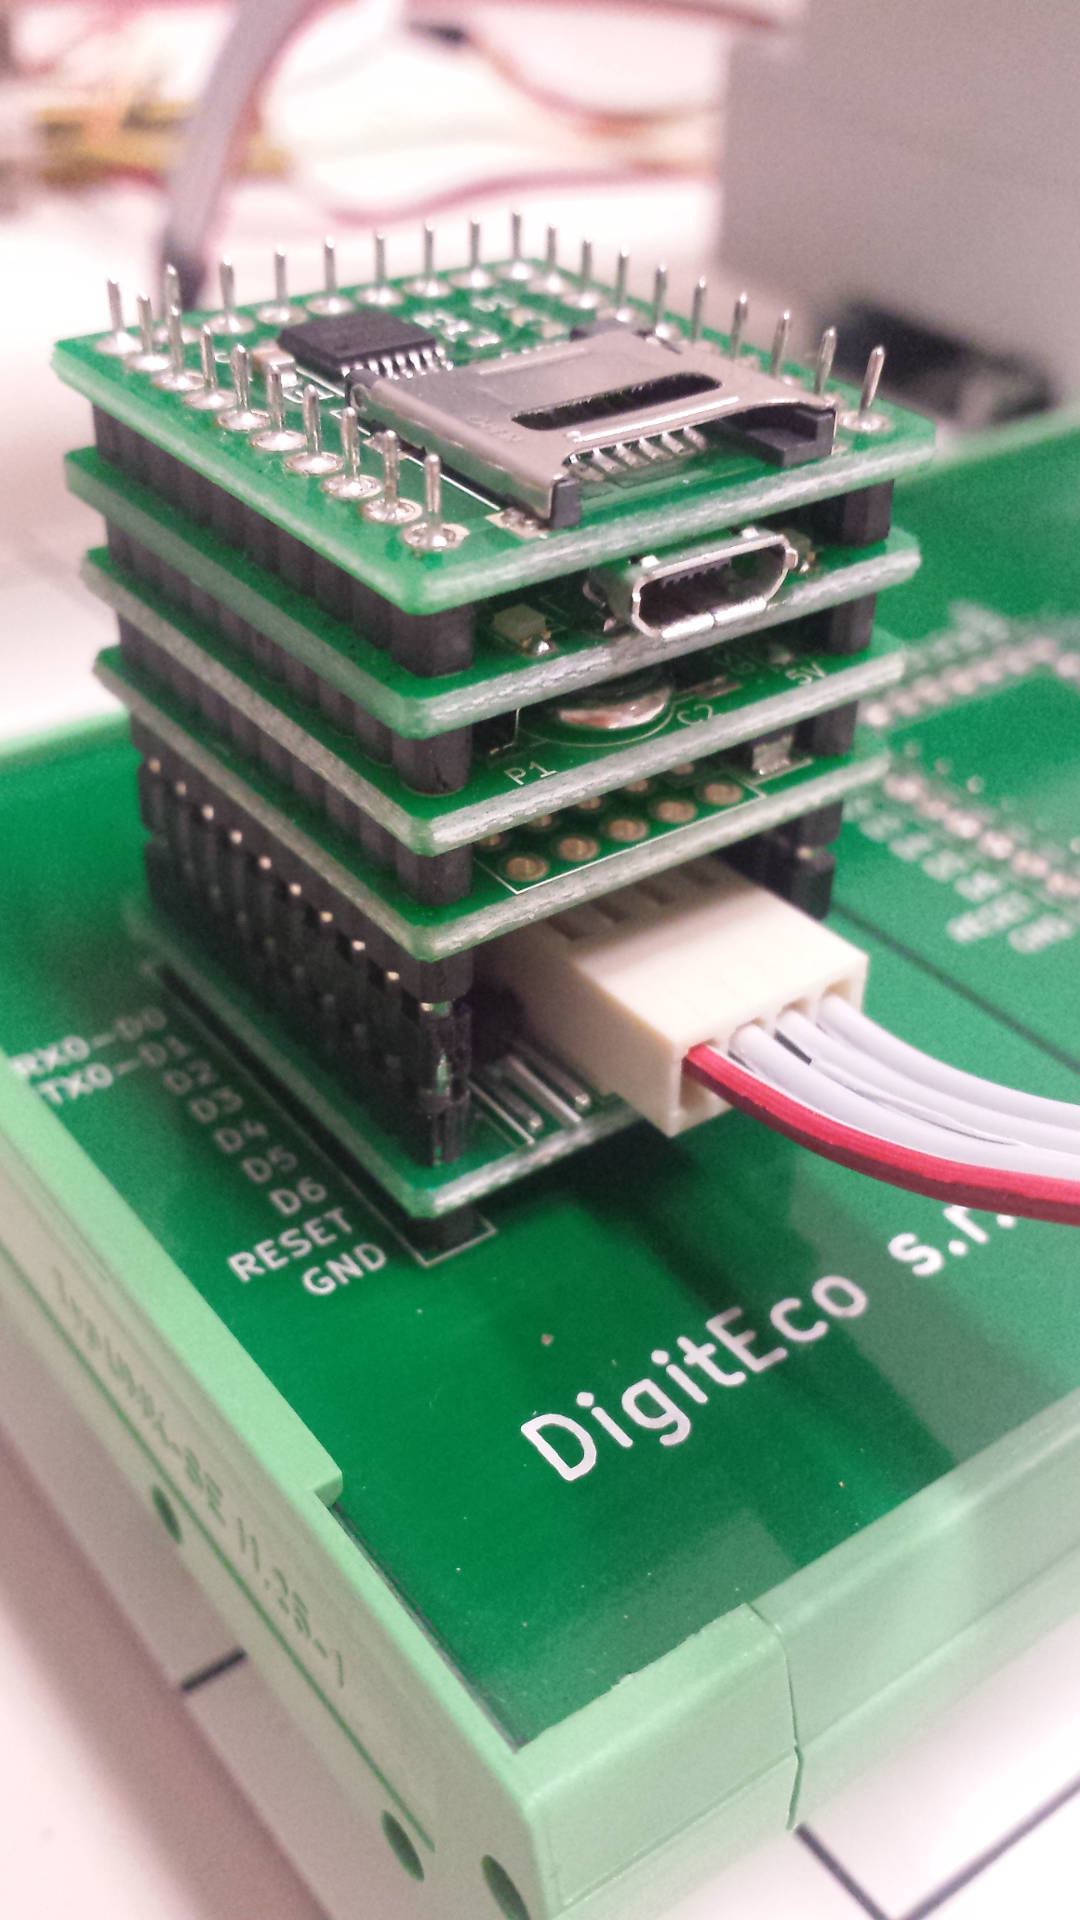
\includegraphics[width=\textwidth,height=\textheight/2,keepaspectratio=true]{passive.jpg}}
\end{DoxyImageNoCaption}
\hypertarget{index_stima_passive_hardware}{}\subsubsection{Hardware}\label{index_stima_passive_hardware}
1) Stima I2\+C-\/\+Base @ 5V / 3.\+3V

2) Stima core+1284 @ 5V / Stima core+644 @ 3.\+3V

3) Stima I2\+C-\/\+R\+TC @ 5V / 3.\+3V

4) Stima F\+T232\+RL\hypertarget{index_stima_passive_software}{}\subsubsection{Software}\label{index_stima_passive_software}
1) open sketch \hyperlink{rmap_8ino}{arduino/sketchbook/rmap/rmap/rmap.\+ino}

2) in \hyperlink{rmap-config_8h}{arduino/sketchbook/rmap/rmap/rmap-\/config.\+h} set S\+T\+I\+M\+A\+\_\+\+M\+O\+D\+U\+L\+E\+\_\+\+T\+Y\+P\+E\+\_\+\+P\+A\+S\+S\+I\+VE in M\+O\+D\+U\+L\+E\+\_\+\+V\+E\+R\+S\+I\+ON define

3) open \hyperlink{sensors__config_8h}{arduino/sketchbook/libraries/\+Rmap\+Config/sensors\+\_\+config.\+h} and set true or false sensors\textquotesingle{}s define and json\textquotesingle{}s define in order to enable or disable relative sensor\textquotesingle{}s driver and library

4) compile and upload firmware

5) short-\/circuit the two configure pins with a jumper and configure it!\hypertarget{index_i2c-th}{}\subsection{S\+T\+I\+M\+A I2\+C-\/\+T\+H\+:}\label{index_i2c-th}
 
\begin{DoxyImageNoCaption}
  \mbox{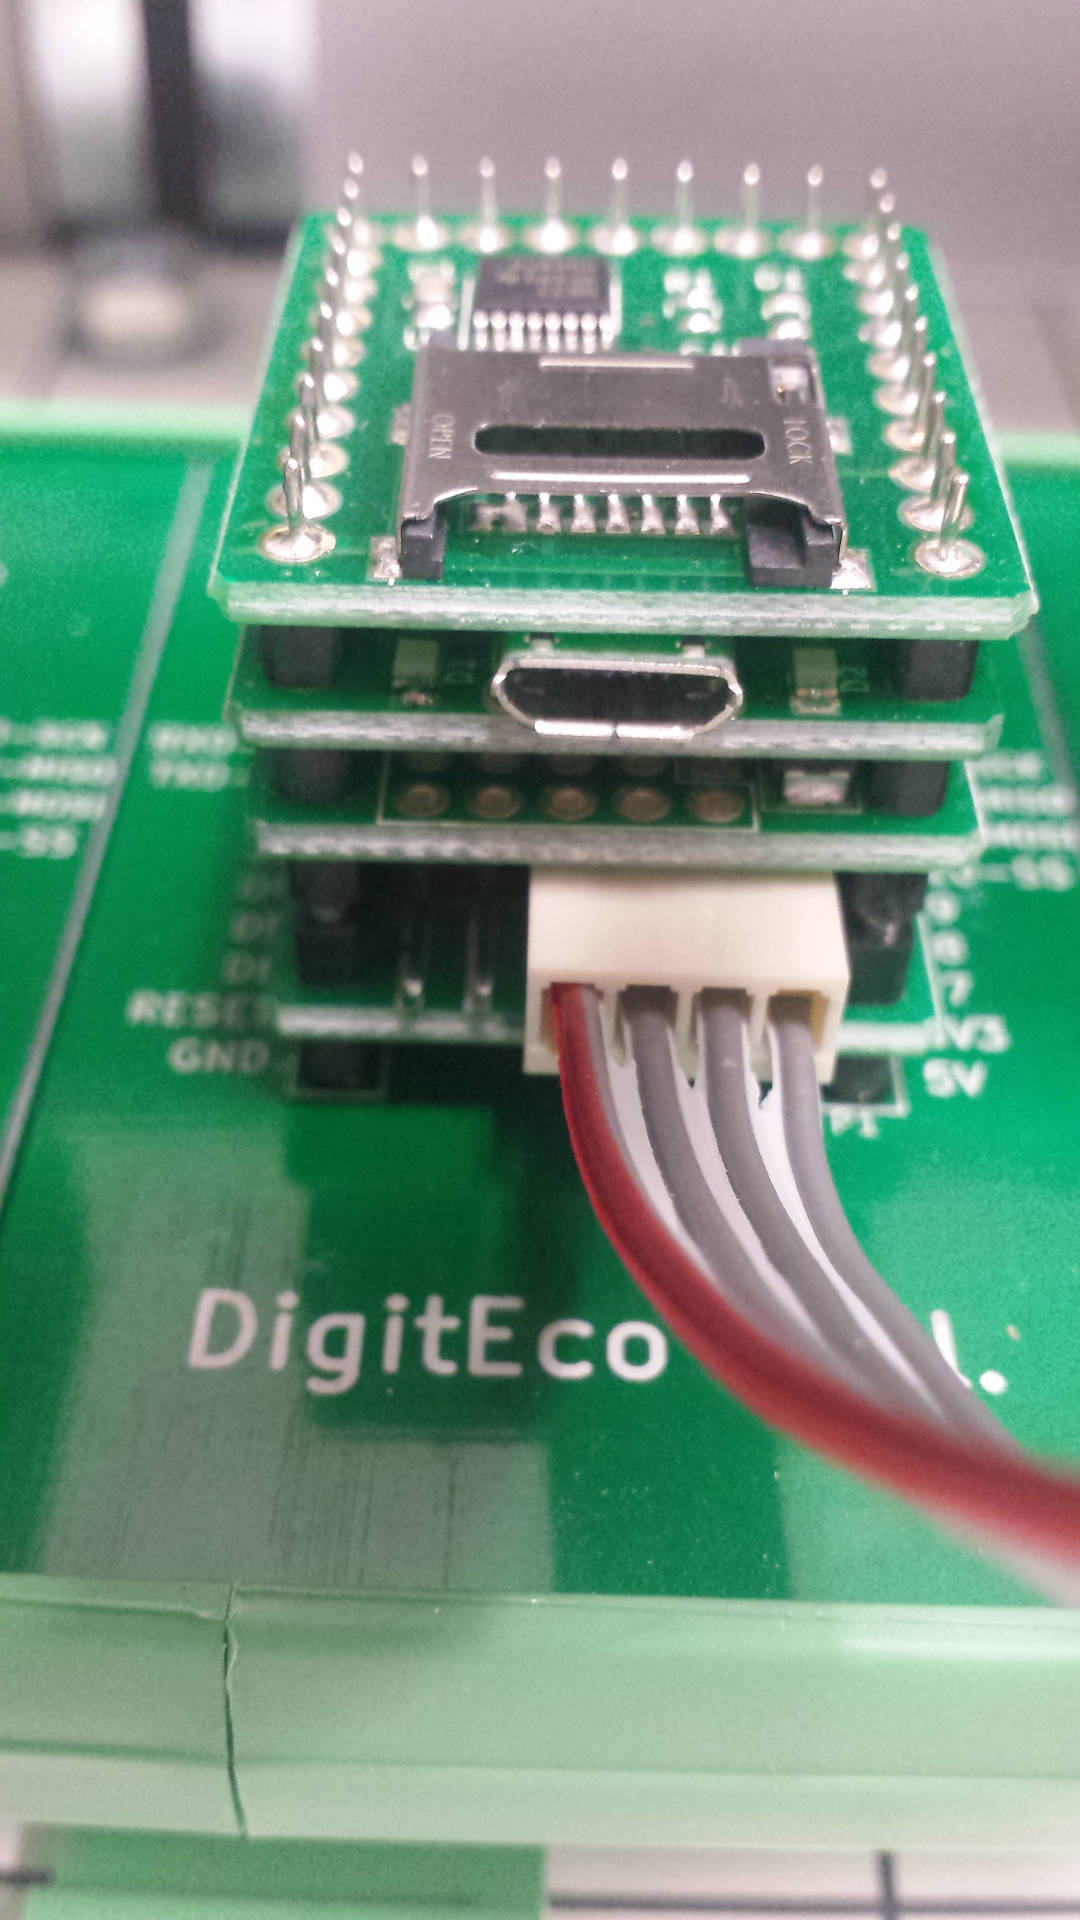
\includegraphics[width=\textwidth,height=\textheight/2,keepaspectratio=true]{th.jpg}}
\end{DoxyImageNoCaption}
\hypertarget{index_stima_i2c_th_hardware}{}\subsubsection{Hardware}\label{index_stima_i2c_th_hardware}
1) Stima I2\+C-\/\+Base @ 3.\+3V

2) Stima core+644 @ 3.\+3V

3) Stima F\+T232\+RL

4) Stima S\+D-\/\+Card\hypertarget{index_stima_i2c_th_software}{}\subsubsection{Software}\label{index_stima_i2c_th_software}
1) open sketch \hyperlink{i2c-th_8ino}{arduino/sketchbook/rmap/i2c-\/th/i2c-\/th.\+ino}

2) open \hyperlink{sensors__config_8h}{arduino/sketchbook/libraries/\+Rmap\+Config/sensors\+\_\+config.\+h} and set true or false sensors\textquotesingle{}s define and json\textquotesingle{}s define in order to enable or disable relative sensor\textquotesingle{}s driver and library

3) compile and upload firmware\hypertarget{index_i2c-rain}{}\subsection{S\+T\+I\+M\+A I2\+C-\/\+Rain\+:}\label{index_i2c-rain}
 
\begin{DoxyImageNoCaption}
  \mbox{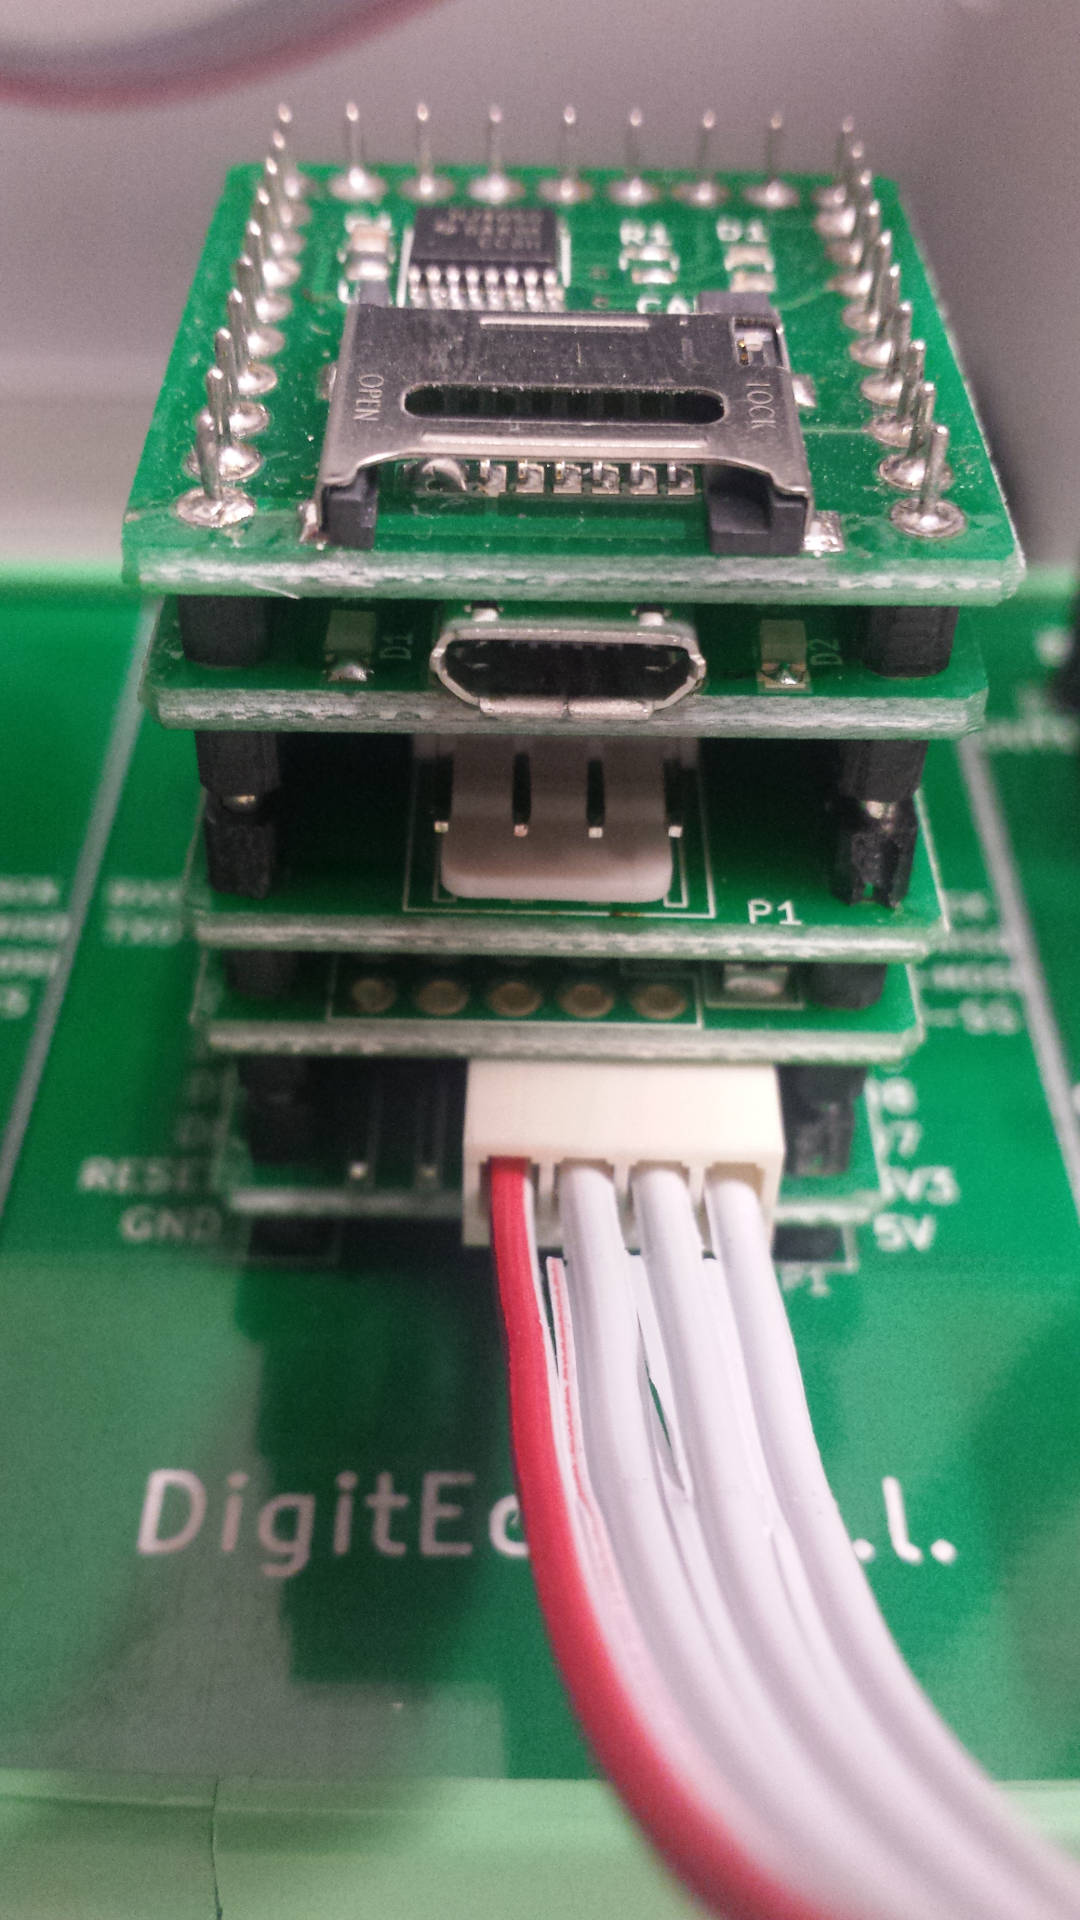
\includegraphics[width=\textwidth,height=\textheight/2,keepaspectratio=true]{rain.jpg}}
\end{DoxyImageNoCaption}
\hypertarget{index_stima_i2c_rain_hardware}{}\subsubsection{Hardware}\label{index_stima_i2c_rain_hardware}
1) Stima I2\+C-\/\+Base @ 3.\+3V

2) Stima core+644 @ 3.\+3V

3) Stima I2\+C-\/\+Digital

4) Stima F\+T232\+RL

5) Stima S\+D-\/\+Card\hypertarget{index_stima_i2c_rain_software}{}\subsubsection{Software}\label{index_stima_i2c_rain_software}
1) open sketch \hyperlink{i2c-rain_8ino}{arduino/sketchbook/rmap/i2c-\/rain/i2c-\/rain.\+ino}

2) open \hyperlink{sensors__config_8h}{arduino/sketchbook/libraries/\+Rmap\+Config/sensors\+\_\+config.\+h} and set false in all sensors\textquotesingle{}s define and json\textquotesingle{}s define

3) compile and upload firmware\hypertarget{index_station}{}\subsection{S\+T\+I\+M\+A Meteo Station assembly}\label{index_station}
 
\begin{DoxyImageNoCaption}
  \mbox{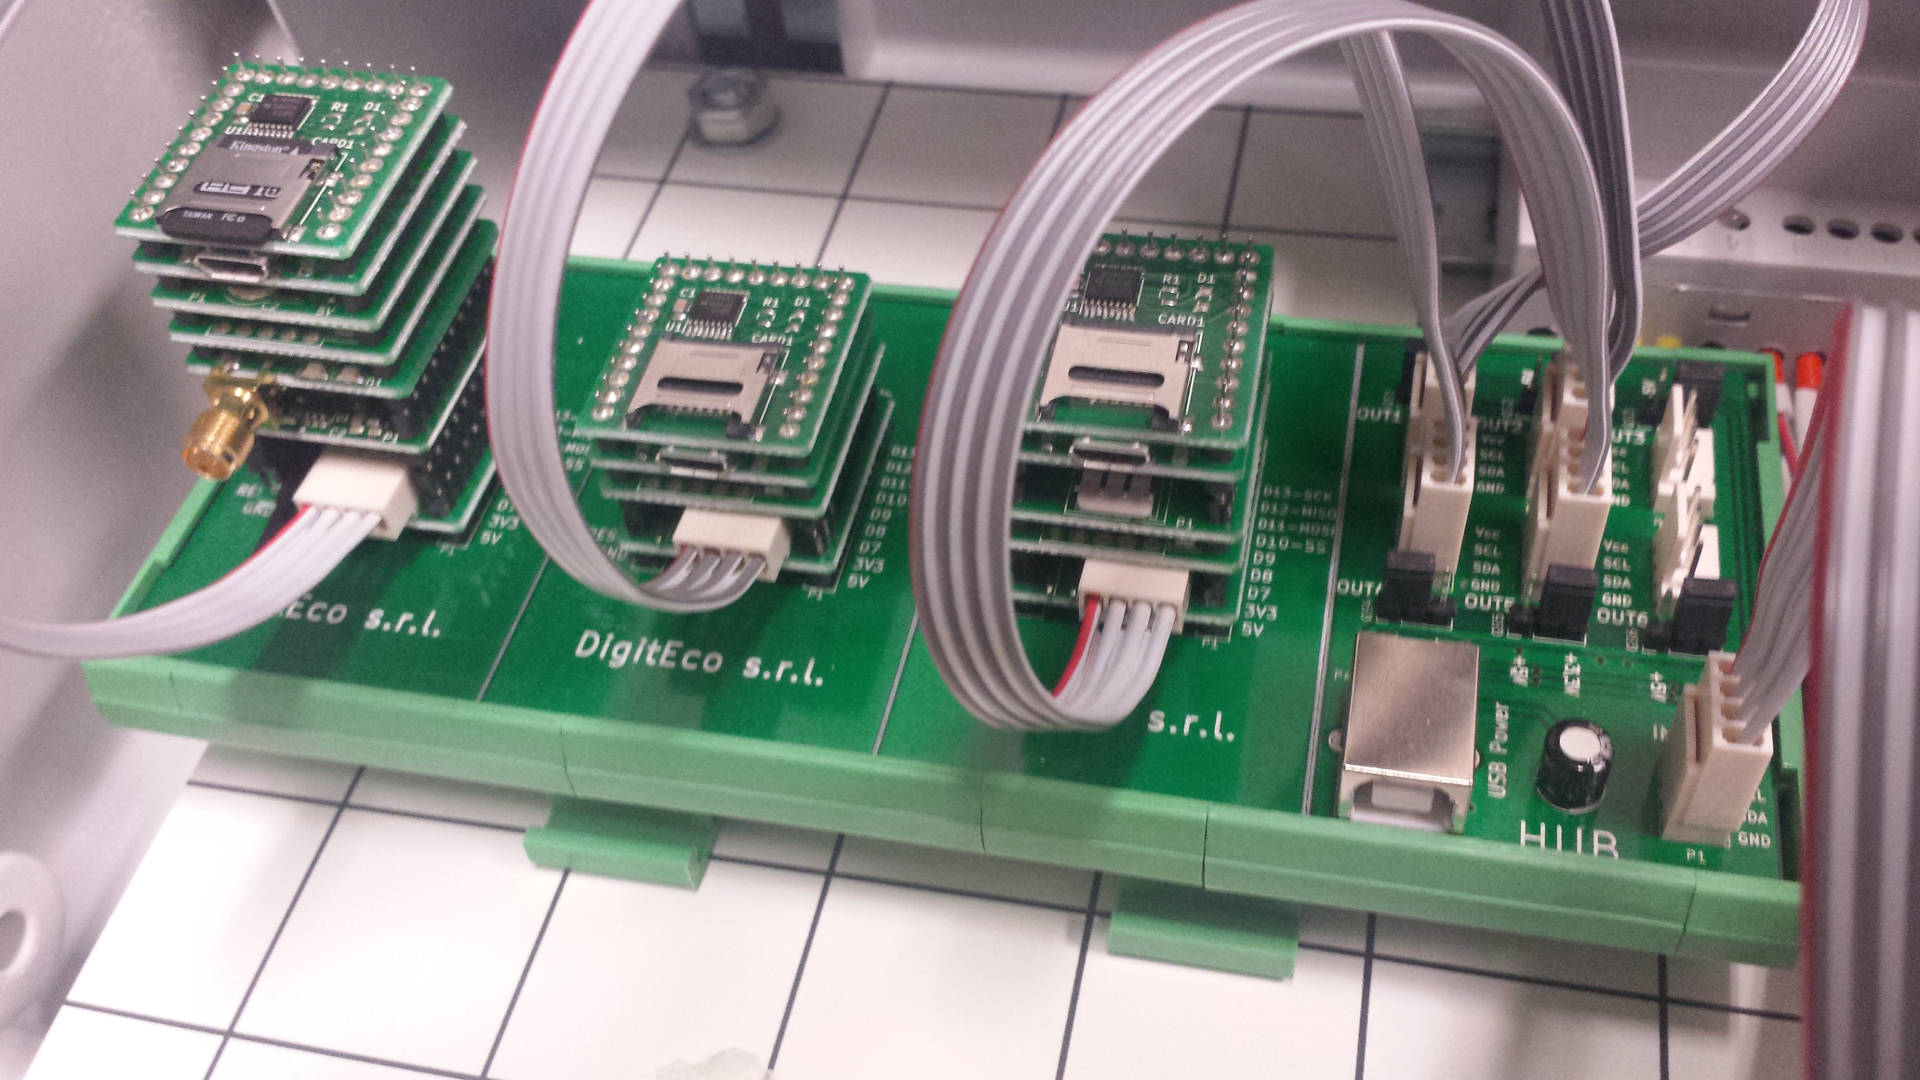
\includegraphics[width=\textwidth,height=\textheight/2,keepaspectratio=true]{station.jpg}}
\end{DoxyImageNoCaption}


1) Stima over Ethernet or Stima over G\+SM

--$>$ connect with a cable at 5V hub port --$>$ in G\+S\+M/\+G\+P\+RS version\+: connect S\+MA antenna and insert a S\+IM card --$>$ in Ethernet version\+: connect ethernet/\+P\+OE cable

2) Stima I2\+C-\/\+TH

--$>$ connect with a cable at 3.\+3V hub port

3) Stima I2\+C-\/\+Rain

--$>$ connect with a cable at 3.\+3V hub port

--$>$ connect at tipping bucket rain on 2 external pins of Stima I2\+C-\/\+Digital

4) I2C sensor\textquotesingle{}s\+:

--$>$ connect with a cable at 3.\+3V or 5V hub port

5) I2C L\+CD Display

--$>$ connect with a cable at 5V hub port

6) Stima I2\+C-\/\+H\+UB

Power up the station through one of the following ways\+:

1) U\+SB power supply with U\+SB type B connector

2) Plug a P\+OE cable into R\+J45 interface (only for ethernet version)

3) 5V DC power supply through hub input port

4) \hyperlink{namespaceDigitecoPower}{Digiteco\+Power} through hub input port with capability of 12V battery backup, solar panel or 12-\/30V DC input source voltage

in that case, the pins on the \hyperlink{namespaceDigitecoPower}{Digiteco\+Power} module are\+:

1) V\+C\+C\+\_\+\+IN\+: 12-\/30V DC input source V\+CC (+)

2) G\+N\+D\+\_\+\+IN\+: 12-\/30V DC input source G\+ND (-\/)

3) V\+C\+C\+\_\+\+B\+AT\+: 12V DC input/otput battery backup V\+CC (+)

4) G\+N\+D\+\_\+\+B\+AT\+: 12V DC input/otput battery backup G\+ND (-\/)

5) Status L\+ED\+: green for battery charged, orange for medium charged battery, red for low battery

6) V\+C\+C\+\_\+\+O\+UT\+: 5V DC output for input hub connector V\+CC (+)

7) S\+CL\+: I2C S\+CL for input hub connector

8) S\+DA\+: I2C S\+DA for input hub connector

9) G\+N\+D\+\_\+\+O\+UT\+: 5V DC output for input hub connector G\+ND (-\/)\hypertarget{index_library}{}\section{Project Library}\label{index_library}
For details, look at the specific library files.\hypertarget{index_rmapconfig}{}\subsection{Rmap\+Config}\label{index_rmapconfig}
This library contains the definitions that are useful for configuring some default values. Below is a list of the files contained therein.

\hyperlink{debug__config_8h}{debug\+\_\+config.\+h}\+: Enable or disable debug in sketch and library

\hyperlink{ethernet__config_8h}{ethernet\+\_\+config.\+h}\+: Ethernet configuration\textquotesingle{}s parameters (IP, D\+H\+CP, delay, ecc..)

\hyperlink{gsm__config_8h}{gsm\+\_\+config.\+h}\+: G\+SM configuration\textquotesingle{}s parameters (A\+PN, username, ecc..)

\hyperlink{hardware__config_8h}{hardware\+\_\+config.\+h}\+: Hardware configuration\textquotesingle{}s parameters (I2C bus clock, ecc..)

\hyperlink{json__config_8h}{json\+\_\+config.\+h}\+: J\+S\+ON configuration\textquotesingle{}s parameters (buffer length)

\hyperlink{lcd__config_8h}{lcd\+\_\+config.\+h}\+: L\+CD configuration\textquotesingle{}s parameters (rows, columns, ecc..)

\hyperlink{mqtt__config_8h}{mqtt\+\_\+config.\+h}\+: M\+Q\+TT configuration\textquotesingle{}s parameters (topic length, buffers length, ecc..)

\hyperlink{ntp__config_8h}{ntp\+\_\+config.\+h}\+: N\+TP configuration\textquotesingle{}s parameters (timezone, server, ecc..)

\hyperlink{sdcard__config_8h}{sdcard\+\_\+config.\+h}\+: S\+D\+C\+A\+RD configuration\textquotesingle{}s parameters (name length, ecc..)

\hyperlink{sensors__config_8h}{sensors\+\_\+config.\+h}\+: Enable or disable sensor driver sensors for specific sketch\hypertarget{index_rmap}{}\subsection{Rmap}\label{index_rmap}
This library contains generic utility features. Below is a list of the files contained therein.

\hyperlink{debug_8h}{debug.\+h} \hyperlink{debug_8cpp}{debug.\+cpp}\+: Debugging functions for print debug message on serial port or L\+CD

\hyperlink{eeprom__utility_8h}{eeprom\+\_\+utility.\+h} eeprom\+\_\+utility.\+cpp\+: E\+E\+P\+R\+OM utility for write and read eeprom

\hyperlink{i2c__utility_8h}{i2c\+\_\+utility.\+h} \hyperlink{i2c__utility_8cpp}{i2c\+\_\+utility.\+cpp}\+: I2C utility for bus recovery

\hyperlink{registers_8h}{registers.\+h}\+: General register\textquotesingle{}s define

\hyperlink{registers-th_8h}{registers-\/th.\+h}\+: I2\+C-\/\+TH register\textquotesingle{}s define

\hyperlink{registers-rain_8h}{registers-\/rain.\+h}\+: I2\+C-\/\+Rain register\textquotesingle{}s define

\hyperlink{rmap__utility_8h}{rmap\+\_\+utility.\+h} \hyperlink{rmap__utility_8cpp}{rmap\+\_\+utility.\+cpp}\+: R\+M\+AP useful functions

\hyperlink{sdcard__utility_8h}{sdcard\+\_\+utility.\+h} \hyperlink{sdcard__utility_8cpp}{sdcard\+\_\+utility.\+cpp}\+: S\+D-\/\+Card useful functions

\hyperlink{stima__module_8h}{stima\+\_\+module.\+h}\+: S\+T\+I\+MA station\textquotesingle{}s definition

\hyperlink{typedef_8h}{typedef.\+h}\+: Useful project typedef\hypertarget{index_sensordriver}{}\subsection{Sensor\+Driver}\label{index_sensordriver}
This library is provided to read measurements from I2C sensors.

\hyperlink{SensorDriverSensors_8h}{Sensor\+Driver\+Sensors.\+h}\+: define list with sensor names in \hyperlink{classSensorDriver}{Sensor\+Driver}

\hyperlink{SensorDriver_8h}{Sensor\+Driver.\+h} \hyperlink{SensorDriver_8cpp}{Sensor\+Driver.\+cpp}\+: \hyperlink{classSensorDriver}{Sensor\+Driver} library files\hypertarget{index_hyt2x1}{}\subsection{H\+Y\+T2\+X1}\label{index_hyt2x1}
This library implements functions for read and configure H\+Y\+T271 and H\+Y\+T221 sensors.

\hyperlink{hyt2x1_8h}{hyt2x1.\+h} \hyperlink{hyt2x1_8cpp}{hyt2x1.\+cpp}\+: H\+Y\+T2\+X1 library files\hypertarget{index_ntp}{}\subsection{N\+TP}\label{index_ntp}
This library implements N\+TP functions for read time over N\+TP server with ethernet client or sim800 client.

\hyperlink{ntp_8h}{ntp.\+h} \hyperlink{ntp_8cpp}{ntp.\+cpp}\+: N\+TP library files\hypertarget{index_pcf8563}{}\subsection{P\+C\+F8563}\label{index_pcf8563}
This library implements P\+C\+F8563 functions for communicate with pcf8563 real time clock.

\hyperlink{pcf8563_8h}{pcf8563.\+h} \hyperlink{pcf8563_8cpp}{pcf8563.\+cpp}\+: P\+C\+F8563 library files\hypertarget{index_sim800}{}\subsection{S\+I\+M800}\label{index_sim800}
This library implements \hyperlink{classSIM800}{S\+I\+M800} functions for communicate with S\+I\+M800\+C/\+S\+I\+M800L G\+S\+M/\+G\+P\+RS module.

\hyperlink{sim800_8h}{sim800.\+h} \hyperlink{sim800_8cpp}{sim800.\+cpp}\+: \hyperlink{classSIM800}{S\+I\+M800} library files

\hyperlink{sim800Client_8h}{sim800\+Client.\+h}\+: \hyperlink{classSIM800}{S\+I\+M800} library interface for Arduino Client.

S\+I\+M800C is fully supported, S\+I\+M800L is partially supported (coming soon...)\hypertarget{index_implemented}{}\subsection{Implemented features}\label{index_implemented}
\hypertarget{index_transport}{}\subsubsection{Transport}\label{index_transport}
o) Serial\+: yes

o) Ethernet\+: partial (basic functions are present but need to interface with Ethernet Client)

o) M\+Q\+TT\+: partial (subscribe functions are present but need to interface with rpc process function)

See Arduino\+Json\+R\+PC library\hypertarget{index_files}{}\subsubsection{S\+D-\/\+Card files}\label{index_files}
On the sdcard there is a file called mqtt\+\_\+ptr.\+txt containing a binary data in uint32\+\_\+t format corresponding to the seconds passed since 00\+:00\+:00 01/01/1970 indicating the last data sent by M\+Q\+TT.

The data is recorded on files (one file for each recording day) named in the format yyyy\+\_\+mm\+\_\+dd.\+txt and each data recorded on sd card is M\+Q\+T\+T\+\_\+\+S\+E\+N\+S\+O\+R\+\_\+\+T\+O\+P\+I\+C\+\_\+\+L\+E\+N\+G\+TH + M\+Q\+T\+T\+\_\+\+M\+E\+S\+S\+A\+G\+E\+\_\+\+L\+E\+N\+G\+TH bytes long (look at the \hyperlink{mqtt__config_8h}{mqtt\+\_\+config.\+h} file).

Each recorded data has the format of the type\+: T\+R\+A\+N\+G\+E/\+L\+E\+V\+E\+L/\+V\+AR \{ “v”\+: V\+A\+L\+UE, “t”\+: T\+I\+ME\}\hypertarget{index_sensordriversensors}{}\subsubsection{Sensor\+Driver\textquotesingle{}s sensors}\label{index_sensordriversensors}
o) A\+D\+T7420 (A\+DT)

o) H\+I\+H6100 (H\+IH)

o) H\+Y\+T221 (H\+YT)

o) H\+Y\+T271 (H\+YT)

o) \hyperlink{namespaceDigitecoPower}{Digiteco\+Power} (D\+EP)

o) I2\+C-\/\+TH (S\+TH, I\+TH, N\+TH, M\+TH, X\+TH)

o) I2\+C-\/\+Rain (T\+BS, T\+BR)

o) I2\+C-\/\+Wind (D\+W1)

other sensors can be easily integrated (see \hyperlink{classSensorDriver}{Sensor\+Driver} library). 